\chapter{Surface Gravity Waves}
\label{kap-waves}
The spectrum of vertical motions of the ocean surface consists of several types 
of waves, covering a broad frequency range.  Wind generated 
waves have periods around $0.25 - 30\,\text{s}$. Locally generated waves, called 
wind sea, are irregular and short crested. While propagating away from the 
generation area, they become long crested and more regular, their periods 
increase. These waves are called swell \citep[][]{holthuijsen2007}. 

Wind generated waves are a main contributor to the energetics in shallow water 
bodies. They generate surface mixed layers and influence the near bed dynamics 
even at considerable water depths. In shallow areas, wave induced maximal 
bottom stress mainly dominates over current induced turbulence 
\citep[][]{jonsson2004}. Consequently, waves play a 
major role in sediment transport and distribution in the Baltic Sea.

In this chapter, a brief description of wind wave properties and processes will 
be given, followed by a discussion of a state of the art wave model, which was 
set up for the Baltic Sea. Finally, the model outcome and its implications on 
the Baltic Sea sediments are analyzed.

\section{Evolution of Waves}

\subsection{Wave Generation by Wind}
Energy is transferred from wind to the waves by wind-induced surface pressure. 
Assuming a harmonic wave propagating in the same direction as the (faster) wind 
blows. The wind field near the water surface is disturbed as indicated in 
\fig{windgen}. Higher air pressure is induced at the windward site of the wave 
crest, where the water surface moves downwards while the wave is propagating, 
and vice versa low air pressure at the leeward site of the wave crest, where 
the sea surface is moving upwards.
\begin{figure}[ht]

 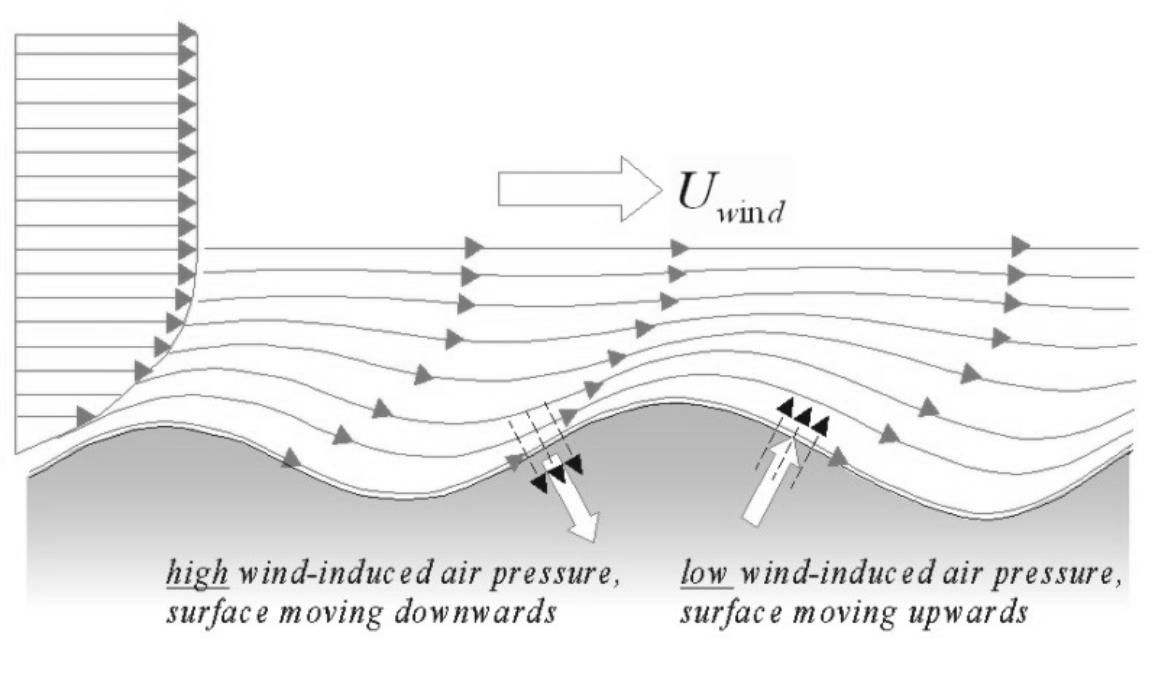
\includegraphics[width=10cm]{bilder/windpressure_sw.png}
 \caption{Wind-pressure distortions over a propagating harmonic wave. Figure 
courtesy \cite{holthuijsen2007}. \label{windgen}}
\end{figure}

This way, the (wave-induced) air pressure distortions amplify the vertical 
movement of the water surface, transfering energy from wind to the wave field. 
This process enforces itself as it is more effective for higher waves. Wave 
growth ends when the wave propagation speed approaches wind speed. It is not 
well understood how initial distortions of the sea surface are generated, but 
fortunately wave growth is not sensitive to the initial wave field.

\subsubsection{Wave Growth Limitation}

Wave growth (in deep water) is not only limited by the wind speed 
$U_{10}$, as mentioned above, but also by the time that wind has been blowing 
and the distance to the coast where the wind comes from. This distance is 
called fetch, and wave height increases the longer the fetch is. Wind duration 
and fetch can be combined to the equivalent fetch, assuming that from the 
moment on that the wind started, a wave component with group velocity $c_g$ has 
travelled a certain distance in wind direction. Wind transfers the same 
energy to the wave component either over a time $t$ or (for an infinitely long 
time period) over a distance
\begin{equation}
 \label{eqFetch}
 F_{eq} = c_g t \cos \theta , 
\end{equation}
where $\theta$ is the wave propagation direction relative to the wind 
direction. This distance is called the equivalent fetch. Sea states where real 
fetch is shorter (longer) than the equivalent one are called fetch-limited 
(duration-limited). At fully developed sea states, the wave phase speed (at 
some peak frequency) has approached $U_{10}$ and wave growth decays.

\subsection{Wave-wave Interaction}

Energy can be transfered between wave components by resonance. This happens, if 
two pairs of waves have the same frequency, wave number vector and direction. A 
pair of waves is a superposition of two waves of different frequencies and wave 
number vectors, which visually form a diamond pattern (\fig{diamond}).
\begin{figure}[ht]
 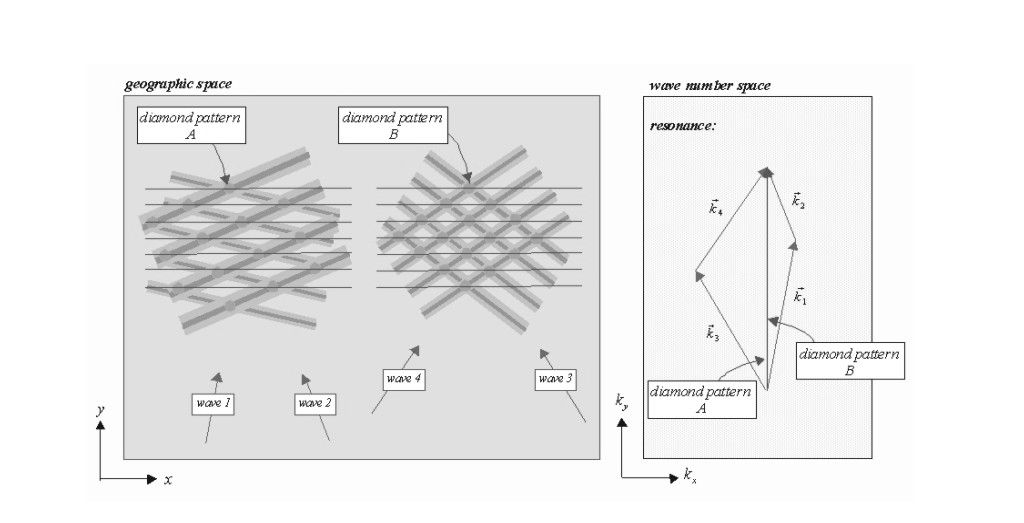
\includegraphics[width=15cm]{bilder/diamond.png}
 \caption{Two pairs of waves, each creating a diamond pattern, fulfill the 
resonance conditions fow quadruplet wave-wave interaction. Figure courtesy 
\cite{holthuijsen2007}. \label{diamond}}
\end{figure}

If two of those diamond patterns fulfill the resonance conditions, energy can 
be distributed among the four waves involved. This mechanism is called 
quadruplet wave- wave interaction. It draws energy from the mid-range 
freequencies and provides it to waves with rather high or low frequencies. 

In shallow water (non-dispersive waves), triad wave-wave interaction is 
possible, where a pair of waves fulfills the above resonance conditions with a 
third wave.

\subsection{Dissipation of Energy}

Wave energy can be dissipated either by white-capping in deep 
water, or by bottom friction and depth-induced breaking in the surf zone. 

White-capping describes the breaking of waves in deep water. This is a 
highly non-linear process which is not understood in detail. Presumably, wave 
steepness and local wind affect the occurence of white-caps, which draw energy 
from waves at frequencies by hindering the upward movement of the sea surface. 
The average dissipative effect of white-capping is rather weak.

\section{Sea State Description}
The most important method 
to describe a sea state is to treat ocean waves as a stochastic process to 
calculate a wave spectrum, from which parameters like wave height are derived. 
One possibility therefore is the random-phase/amplitude model, described in 
detail in \cite{holthuijsen2007}: The time series of surface elevation $ \eta 
(t)$ is assumed to be a superposition of $N$ sinusoidal waves, each with a 
distinct frequency $f_i$, amplitude $a_i$ and phase $\alpha_i$, written as
\begin{equation}
 \label{sinussum}
 \eta(t) = \sum_{i=1}^N a_i \cos (2\pi f_i t + \alpha_i).
\end{equation}
Considering $a_i$ and $\alpha_i$ to be independent random variables, 
probability density functions for both can be derived from observations. For 
waves in sufficiently deep water which are not too steep, it was found that the 
phase is uniformly distributed (and can therefore be omitted in the wave 
spectrum), while the amplitude is Rayleigh distributed with expected value 
$E\{a_i\} = \mu_i$ for each frequency $f_i$. The function $f_i \rightarrow 
E\{a_i\}$ is called the amplitude spectrum and already contains all 
(non-directional) information of the sea state. A more meaningful 
characterization is, however, the variance spectrum $f_i \rightarrow E\{a_i^2 
\slash 2\}$, as the variance is proportional to the wave energy contained in 
each frequency, with the proportionality constant $\rho g$. Here, $\rho$ denotes 
density of the water and $g$ the gravitational acceleration. By scaling the 
variance of each discrete frequency with the frequency bin $\Delta f$ (i.e. the 
size of the frequency resolution) and formally assuming infinitely small 
frequency bins, the variance density spectrum is obtained. Multiplied by the 
factor $\rho g$, this is the energy density spectrum:
\begin{equation}
 \label{vardensspec}
 E(f) = \rho g \lim_{\Delta f \rightarrow 0} \frac{1}{\Delta f} E\{\frac{1}{2} 
a_i^2\}.
\end{equation}
For a harmonic wave, i.e. all wave energy is contained in one distinct 
frequency, $E(f)$ reduces to a delta function. For more irregular waves, the 
energy density spectrum broadens. 

The shape of this spectrum is not at all arbitrary, but was found to have 
rather uniform characteristics under similar conditions. For a fully 
developed sea state, the Pierson-Moskowitz (PM) spectrum was derived: 
\begin{equation}
 \label{PMspectrum}
 E_{PM}(f) = \underbrace{\alpha_{PM}g^2(2 
\pi)^{-4}f^{-5}}_{f^{-5}\text{-tail}} \underbrace{\exp \left[ - \frac{5}{4} 
\left( \frac{f}{f_{PM}} \right)^{-4} \right]}_{\text{low-freq. cut-off}}.
\end{equation}
The $f^{-5}$ - tail comes from a dimensional argument under the assumption, 
that wave breaking limits the spectra on the high frequency side, and that this 
process is determined only by the gravitational acceleration and the wave 
frequency itself. Therefore, $E(f) \sim g^2f^{-5}$ at high frequencies. At a 
peak frequency $f_{PM}$, depending on the wind speed, a smooth low-frequency 
cut-off is imposed. From observations, an energy scale of $\alpha_{PM} = 
0.0081$ was derived.

The PM spectrum describes a fully developed sea state, i.e. 
constant wind conditions being present until sea state becomes stationary and 
no fetch limitation is assumed. Observed sea states rarely fulfill these 
assumptions, and during an extensive study, the JONSWAP (Joint North Sea wave 
Project, \cite{hasselmann1974}) spectrum for young sea states was designed:
\begin{equation}
 \label{JONSWAPspectrum}
 E_{JONSWAP}(f) = \underbrace{\alpha g^2(2 
\pi)^{-4}f^{-5} \exp \left[ - \frac{5}{4} \left( \frac{f}{f_{\text{peak}}} 
\right)^{-4} \right]}_{\text{PM shape}} \underbrace{\gamma^{\exp \left[ - 
\frac{1}{2} \left( \frac{f}{\sigma f_{\text{peak}}} \right)^2 \right]}}_{G(f)}.
\end{equation}
Here, the PM spectrum was down-scaled with a higher peak frequency 
$f_\text{peak}$ and a smaller energy scale $\alpha$ (which depends on the 
$f_\text{peak}$ now) to maintain the shape of the PM spectrum. $G(f)$ is a peak 
enhancement function, which amplifies and narrows the spectrum around the peak 
frequency. Hereby, $\gamma$ and $\sigma$ control height and width of the peak, 
respectively. 

The JONSWAP spectrum was found to be a good generalization of observed wave 
energy spectra, not only for idealized fetch-limited conditions but also for 
arbitrary wind conditions. Reason for that is that wave-wave interaction (see 
above) distributes energy among wave frequencies in a way that stabilizes the 
shape of the JONSWAP spectrum. 

The energy spectra discussed above are one dimensional, only depending on wave 
frequency. No information about the propagation direction of waves are 
included. To completely describe a sea state, the energy spectrum $E(f,\theta)$ 
has to be extended by informations about how energy is distributed among waves 
traveling in propagation direction $\theta$.

\section{Third Generation Wave Model SWAN}

The open source wave model SWAN, an acronym for \textbf{S}imulating \textbf{WA}ves \textbf{N}earshore, is a wave model optimized for applications in coastal waters. As the spatial resolution of model domains in coastal regions is often very fine to capture smaller features in topography, SWAN has an implicit propagation scheme implemented, assuring numerical stability even for timesteps, that violate the CFL criterion. 

The central equation that is solved for every timestep at every grid point is 
the action balance equation, that accounts not only for the energy distributions 
in the wave frequency space but also for frequency shifts by wave-current 
interaction. The action density $N=N(\sigma,\theta; x,y,t)$ is therefore 
dependent on the relative radian frequency $\sigma$, which is the shifted 
frequency in a system moving with the current:
\begin{equation}\label{ebe}
 \frac{\partial N}{\partial t} + \frac{\partial c_{g,x} N}{\partial x} + \frac{ \partial c_{g,y} N}{\partial y} + \frac{\partial c_{\theta} N}{\partial t} + \frac{\partial c_{\sigma} N}{\partial \sigma}= \frac{S_{in} + S_{nl} + S_{wc}}{\sigma},
\end{equation}
where the source terms on the right hand side refers to energy input by wind, 
nonlinear wave -- wave interaction and energy dissipation by white capping. $t, 
x ,y$ are time and spatial directions, $\theta$ is the direction of wave energy 
propagation and $c_{g,x}, c_{g,y}$ are the group speed in each spatial 
direction. The fifth term on the left had side represents the frequency shift by 
ambient currents.

In the absence of currents, this action balance equation reduces to the energy balance equation.
\begin{equation}\label{ebe}
 \frac{\partial E}{\partial t} + \frac{\partial c_{g,x} E}{\partial x} + \frac{ \partial c_{g,y} E}{\partial y} + \frac{\partial c_{\theta} E}{\partial t} = S_{in} + S_{nl} + S_{wc}.
\end{equation}
All equations in the following will be noted, consistent with the action balance equation, in terms of the relative radian frequency $\sigma$. Although various formulations for the different mechanisms below are implemented in SWAN, only the ones used in the setup for the Baltic Sea in chapter \ref{balticswan} are described.

\subsection{Wave generation by wind}

Wind data is provided to the model as the wind speed and direction at 10 m elevation, $U_{10}$. This value is converted to a friction velocity via
\begin{equation}
 u_\ast^2 = C_D U_{10}^2.
\end{equation}
Before version 41.01 of SWAN, the wind drag coefficient was linearly dependent on the wind speed with an imposed lower limit. This formulation was found to overestimate $C_D$ for strong winds. Therefore, \cite{zijlema2012} fitted a second-order polynomial to nearly 5000 observed wind drag coefficients in dependence of the wind speed and came up with 
\begin{equation}
 C_D = \left( 0.55 + 2.97 \dfrac{U_{10}}{U_{ref}} - 1.49 \left( \dfrac{U_{10}}{U_{ref}} \right)^2 \right) \times 10^{-3} ,
\end{equation}
where $U_{ref} = 31.5 \, \text{m s}^{-1}$ is the wind speed at which $C_D$ is maximal.

The source term for energy input by wind includes two mechanisms:
\begin{equation}\label{gen}
 S_{in} (f, \theta) = \alpha + \beta E(f,\theta),
\end{equation}
where $\alpha$ is the initial wave growth, parameterized with the following empirical expression by Cavaleri and Malanotte--Rizzoli
\begin{equation}
 \alpha = 
 \begin{cases}
  \dfrac{1.5 \cdot 10^{-3}}{g^2 2 \pi} \left(u_\ast \cos{(\theta - \theta_{wind})}\right)^4 G & \text{for } |\theta - \theta_{wind}| \le 90^\circ  \\
  0 & \text{for } |\theta - \theta_{wind}| \textgreater 90^\circ  \\
 \end{cases}
\end{equation}
where $G$ is a cut-off function to avoid wave growth at frequencies below the Pierson--Moskowitz frequency, $g$ the gravitational acceleration and $\theta_{wind}$ is the wind direction. 

Another implemented approach to quantify the initial wave growth is to impose the JONSWAP spectrum for young sea states. The non-dimensional peak wave frequency $\tilde{f}_{peak} = f_{peak} U_{10} / g$ is thereby derived using the spatial step size at each point as fetch $F$ with an empirical equation by \cite{kahma1992} for short fetch lengths:
\begin{equation}
 \tilde{f}_{peak} = 2.18 \tilde{F}^{-0.27},
\end{equation}
where $\tilde{F} = g F / U_{10}^2$. All other coefficients in the JONSWAP energy spectrum equation are derived from this peak frequency \citep[][]{holthuijsen2007}, and  wave directions are assumed to be $\cos^2$ distributed.

For the exponential wave growth term $\beta$ in \eqref{gen} the classical expression of \citep[][]{komen1984} is used:
\begin{equation}
 \beta = \max \{ 0,0.25 \frac{\rho_{air}}{\rho_{water}} \left[28 \frac{u_\ast}{c} \cos(\theta - \theta_{wind}) -1 \right] \} \sigma,
\end{equation}
with the phase velocity $c$ and $\rho_{air}$ and $\rho_{water}$ the densities of air and water.

\subsection{Nonlinear wave -- wave interaction}

The calculation of quadruplet wave-wave interaction requires large 
computational resources because of the high number of possible quadruplet 
constellations. It is calculated with the discrete-interaction approximation 
(DIA) by \citep[][]{hasselmann1985}. Only two constellations of wave quadruplets 
are considered to interact. The frequencies must fulfill
\begin{align*}
 \sigma_1 &= \sigma_2 = \sigma \\
 \sigma_3 &= 1.25 \sigma = \sigma^+ \\
 \sigma_4 &= 0.75 \sigma = \sigma^- .\\
\end{align*}
The wave directions must be equal for the waves with frequency $\sigma$, while the waves with frequencies $\sigma_3$ and $\sigma_4$ lie at angles of $\theta_1 = -11.5^\circ \; \left[ \text{or } \theta_1 = 11.5^\circ \right]$ and $\theta_2 = 33.6^\circ \; \left[ \text{or } \theta_2 = -33.6^\circ \right]$  to them. The contribution for each quadruplet to the source term $S_{nl}$ in Eq. (\ref{ebe}) is:
\begin{equation}
 S_{nl4}^\ast (\sigma, \theta) = 2 \delta S_{nl4} (\alpha_1 \sigma, \theta) - \delta S_{nl4} (\alpha_2 \sigma, \theta) - \delta S_{nl4} (\alpha_3 \sigma, \theta),
\end{equation}
where for $i \in \{1,2,3\}$
\begin{align*}
 \delta S_{nl4} ( \alpha_i \sigma, \theta ) = & 2.12 \cdot 10^{(-4)} \sigma^{11} \cdot [ ( 0.41 E(\alpha_i \sigma^+, \theta)E^2(\alpha_i \sigma, \theta) \\
 &+ 3.16 E(\alpha_i \sigma^-, \theta) ) - 54.6 E(\alpha_i \sigma, \theta) E(\alpha_i \sigma^+, \theta) E^2(\alpha_i \sigma^-, \theta) ] .
\end{align*}
The coefficients are $\alpha_1 = 1, \, \alpha_2 = 1.25, \, \alpha_3 = 0.75$. 

The above holds for infinite water depth and must be multiplied with a scaling 
factor 
\begin{equation}
 R ( \tilde{k}d ) = \max \{ 1+ \frac{22}{3}\tilde{k}d \left( 1-\frac{6}{7} \tilde{k}d \right) \times \exp(-1.25 \tilde{k}d) , 4.43 \} ,
\end{equation}
depending on the mean wave number $\tilde{k}$ and the the water depth $d$ to obtain the finite depth contribution to the source term for nonlinear wave -- wave interaction.

\subsection{Dissipation}

Wave energy is dissipated by white -- capping. The representation of this process originates from \citep[][]{hasselmann1974}:
\begin{equation}
 S_{wc} (\sigma, \theta ) = - 2.36 \cdot 10^{-5} \frac{k}{\tilde{k}} \left( \frac{\tilde{s}}{\tilde{s}_{PM}} \right)^4 \frac{\tilde{\sigma}}{\tilde{k}} k E(\sigma, \theta),
\end{equation}
with $\tilde{s} = \tilde{k} \sqrt{m_0}$ being the overall wave steepness, $k$ 
the wave number, $\tilde{\sigma}$ the mean wave frequency and $\tilde{s}_{PM} = 
\sqrt{3.02 \times 10^{-3}}$ the overall wave steepness of the Pierson -- 
Moskowitz spectrum.


\subsection{Wave model setup for the Baltic Sea}\label{balticswan}

The SWAN wave model version 41.01 was set up for the Baltic Sea including a 
nesting in the area of the German coastal sea. For the whole Baltic Sea, a grid 
resolution of $0.5^\circ \times 0.1^\circ $ in Latitude and Longitude was chosen 
in a domain reaching from $53.5^\circ \text{N } 9^\circ \text{E}$ to $66^\circ 
\text{N } 31^\circ \text{E}$. This includes the Kattegat, the passage from the 
Baltic to the North Sea, where boundary conditions were prescribed in the east: 
A constant JONSWAP spectrum with a wave height of $1$ m, a period of $5$ s and 
peak wave direction of $90^\circ$ with a high directional spreading. The passage 
from the North to the Baltic sea is very shallow, so the boundary conditions 
have negligible influence on the model outcome. Wave frequency range was set to 
0.1 to 1.8 Hz, which mirrors the actual wave frequencies in the Baltic 
Sea \citep[][]{balticsea}, with a resolution of $42$ frequency bins. 
Computations included a spin-up time of $10$ days, sufficient for wave modeling 
and were performed for the years 2013 and 2014. The model was forced by wind 
data from the German Weather Service (DWD), the computational time step was $1$ 
hour (note that the propagation scheme implemented in SWAN is implicit, so the 
time step is not restricted by numerical issues). 

The nesting area reached from $53.5^\circ \text{N } 10^\circ \text{E}$ to 
$55.5^\circ \text{N } 15^\circ \text{E}$, including the Western German coastal 
seas. Spatial resolution was $0.01^\circ \times 0.025^\circ $ in Latitude and 
Longitude and the computational time step was set to $15$ minutes. Boundary 
conditions came from the Baltic Sea model and all parameters were left 
unchanged.

In \fig{verify} the significant wave height calculated with the wave model was 
compared to data obtained with a wave rider buoy. The significant wave height 
is defined as the average wave height of the highest one-third of the waves. 
This value matches the visually observed wave height best and can be calculated 
from the zeroth-order moment if the variance density spectrum $m_0$ via 
$H_{sign} = 4 \sqrt{m_0}$.
\begin{figure}[ht]
 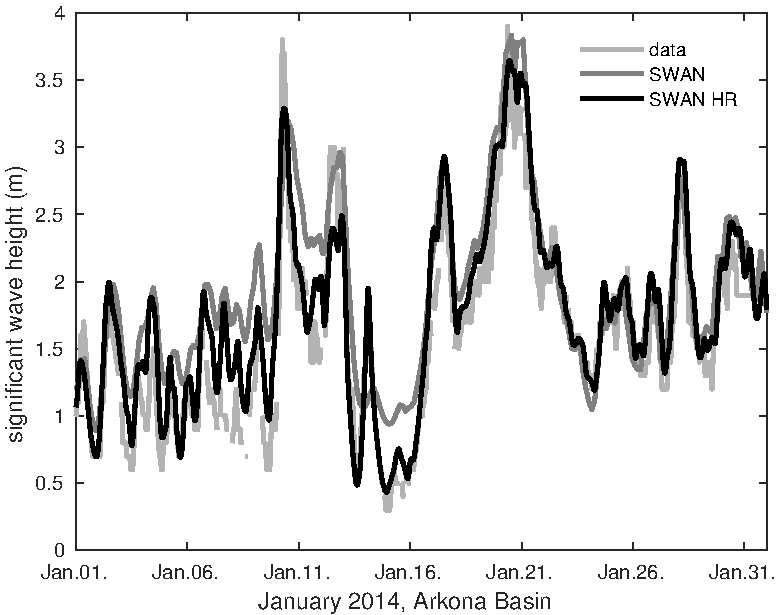
\includegraphics[width=9cm]{bilder/januar.pdf}
 \caption{Significant wave height calculated with the SWAN wave model (HR 
refers to the high resolved nested run) and measured wave height from the 
Arkona wave rider buoy.\label{verify}}
\end{figure}

In the context of a Master Thesis \citep[][]{masterarbeitronja}, the model 
setup for 2013 (still using the previous version SWAN 40.91AB) was 
extensively tested for numerical convergence and compared to measured data on 
several locations in the Baltic Sea. Wave parameters like significant wave 
height were in good agreement with obtained data, even in areas with complex 
topography.

\section{Wave climate of the Baltic Sea}	

\subsection{Observations and Model Outcome}

\subsection{Implications on Sediment Transport}